\frame{TODO}: finish integrating SM revisions
\par
\color{gray}
In this section we introduce a unified system of equations
to describe risk group turnover
in deterministic epidemic models with heterogeneity in risk.
% JK: this "with heterogeneity in risk" feels a little redundant?
We then describe how the unified approach can be used in practical terms,
based on different assumptions and data available for parameterizing turnover in risk.
We then conclude by framing previous approaches to this task using the proposed system.
% ==================================================================================================
\subsection{Notation}
Consider a population divided into $G$ risk groups.
We denote the number of individuals in risk group $i \in [1, \dots, G]$ as $x_i$
and the set of all risk groups as $\bm{x} = \{x_1, \dots, x_G\}$.
The total population size is $N = \sum_i {x_i}$,
and the relative population size of each group
is denoted as $\hat{x}_i = x_i / N$.
Individuals enter the population at a rate $\nu$ per year,
and exit at a rate $\mu$ per year.
We assume that individuals entering into the population
originate from another exogenous population
$\bm{e} = \{e_1, \dots, e_G\}$.
We make this assumption so that the exogenous population $\bm{e}$
may have different relative risk group sizes from the system population $\bm{x}$.%
\footnote{We could equivalently stratify the rate of entry $\nu$ by risk group
  while keeping the exogenous population $\bm{e}$
  equal to the system population $\bm{x}$.
  However, we find this formulation more difficult to work with
  in the subsequent sections.}
That is, $\hat{e}_i$ may not necessarily equal $\hat{x}_i$.
However, since the entry rate $\nu$ is relative to the size $N$ of population $\bm{x}$,
it will be convenient and otherwise inconsequential to assume that population $\bm{e}$
also has size $N$.
That way, the total number of individuals
entering into population $\bm{x}$ per year is given by $\nu N$,
and the number of individuals
entering into group $x_i$ specifically is given by $\hat{e}_i \nu N$.
\par
Turnover transitions may then occur between any two groups, in either direction.
Therefore we denote the turnover rates as a $G \times G$ matrix $\phi$.
The element $\phi_{ij}$ corresponds to the proportion of individuals in group $x_i$
who move from group $x_i$ to group $x_j$ each year.
An example matrix is given in Eq.~(\ref{eq:phi}),
where we write the diagonal elements as $*$ since they represent
transitions from a group to itself.
\begin{equation}\label{eq:phi}
\phi = \left[\begin{array}{cccc}
	         *          & x_1  \rightarrow x_2 & \cdots & x_1 \rightarrow x_G \\[0.5em]
	x_2 \rightarrow x_1 &          *           & \cdots & x_2 \rightarrow x_G \\[0.5em]
	      \vdots        &        \vdots        & \ddots &       \vdots        \\[0.5em]
	x_G \rightarrow x_1 & x_G \rightarrow x_2  & \cdots &          *
\end{array}\right]
\end{equation}
Risk groups, transitions, and the associated rates
are also shown for $G = 3$ in Figure~\ref{fig:system}.
\begin{figure}
  \centering
  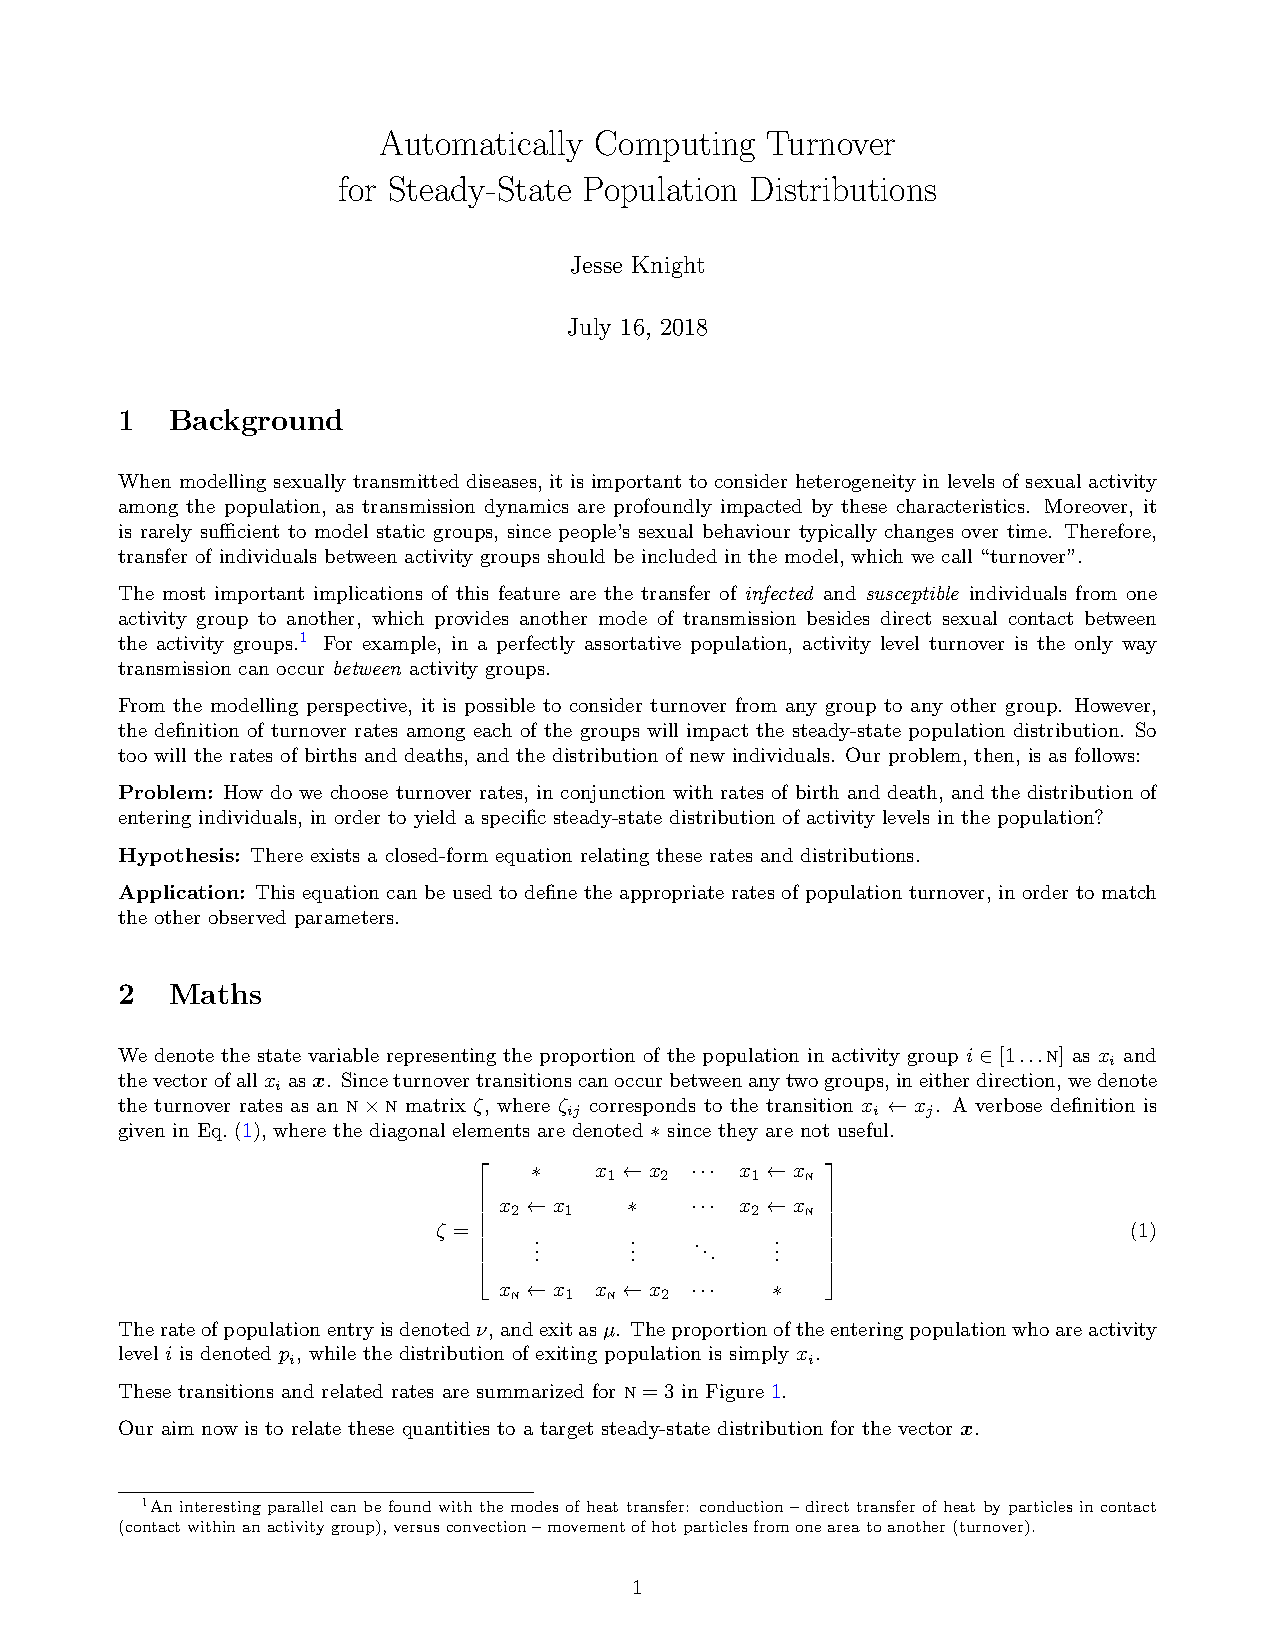
\includegraphics[width=0.5\linewidth]{turnover}
  \caption{System of risk groups and flows between them for $G = 3$}
  \label{fig:system}
\end{figure}
% ==================================================================================================
\subsection{Parameterization}\label{ss:params}
Next, we consider the goal of constructing a system like the one introduced above
which reflects the risk group dynamics observed in a specific context.
We assume that the relative sizes of the risk groups in the model ($\bm{\hat{x}}$)
are already known, and should remain constant over time.
Thus, what remains is to estimate the values of the parameters:
$\nu$, $\mu$, $\bm{\hat{e}}$, and $\phi$,
using commonly available sources of data.
% --------------------------------------------------------------------------------------------------
\subsubsection{Total Population Size}\label{sss:params-nu-mu}
The total population size $N(t)$ is a function of
the rates of population entry $\nu(t)$ and exit $\mu(t)$, given an initial size $N_0$.
We allow the proportion entering the system to vary by risk group via $\bm{\hat{e}}$,
while the exit rate has the same value for each group.
We assume that there is no disease-attributable death.
Because the values of $\nu$ and $\mu$ are the same for each risk group, 
they can be estimated independent of
$\bm{\hat{x}}$, $\bm{\hat{e}}$, and $\phi$.
\par
The difference between entry and exit rates
defines the rate of population growth:
\begin{equation}\label{eq:growth-G}
\mathcal{G}(t) = \nu(t) - \mu(t) 
\end{equation}
The total population may then be defined using an initial population size $N_0$ as:
% SM: suggest including citation for equation (3) and (4)
%     as they have been shown/used before from demography
% JK: (4) for sure, but I had trouble finding (3)
%     had to derive it myself, with a little online help...
%     https://math.stackexchange.com/questions/2361180
\begin{equation}\label{eq:growth-vary}
  N(t) = N_0 \exp{\left(\int_{0}^{\,t}{\log\big(1+\mathcal{G}(\tau) \big)d\tau}\right)}
\end{equation}
which, for constant growth, simplifies to the familiar expression~\citep{Malthus1798}:
\begin{equation} \label{eq:growth-const}
  N(t) = N_0 {(1 + \mathcal{G})}^{t}
\end{equation}
Census data, such as \citep{WorldBank}, can be used to source
the total population size in a given geographic setting over time $N(t)$,
thus allowing Eqs.~(\ref{eq:growth-vary})~and~(\ref{eq:growth-const})
to be used to estimate $\mathcal{G}(t)$.
\par
If the population size is assumed to be constant,
then $\mathcal{G}(t) = 0$ and $\nu(t) = \mu(t)$.
If population growth occurs at a stable rate, then
$\mathcal{G}$ is fixed at a constant value
which can be estimated via Eq.~(\ref{eq:growth-const})
using any two values of $N(t)$, separated by a time interval $\tau$:
\begin{equation}\label{eq:growth-backwards}
\mathcal{G}_{\tau} = {\frac{N(t+\tau)}{N(t)}}^{\frac{1}{\tau}} -1
\end{equation}
If the rate of population growth $\mathcal{G}$ varies over time,
then Eq.~(\ref{eq:growth-backwards}) can be reused for consecutive time intervals,
and the complete function $\mathcal{G}(t)$ approximated piecewise by constant values.
The piecewise approximation can be more feasible
than exact solutions using Eq.~(\ref{eq:growth-vary}),
and can reproduce $N(t)$ accurately for small enough intervals $\tau$,
such as one year.
% SM: the above sentence would benefit from a citation for
%     'feasibility' and 'reproducing accurately' otherwise it may be considered editorializing
% JK: I softened 'is generally more feasible' to 'can be more feasible'
%     but I don't really know where to find a citation on the accuracy of
%     exponential piecewise approximations of variable rate exponential growth.
\par
Now, given a value of $\mathcal{G}(t)$,
either $\nu(t)$ must be chosen and $\mu(t)$ calculated using Eq.~(\ref{eq:growth-G}),
or $\mu(t)$ must be chosen, and $\nu(t)$ calculated.
Most modelled systems assume
a constant duration of time that individuals spend in the model $\delta(t)$~\citep{Anderson1991}
%However, it is common to assume a constant duration of individuals in the model $\delta(t)$,
which is related to the rate of exit $\mu$ by:
\begin{equation} \label{eq:duration-model}
\delta(t) = \mu^{-1}(t)
\end{equation}
In the context of sexually transmitted infections, the duration of time usually reflects
the average sexual life-course of individuals from age 15~to~50 years,
such that $\delta = 35$ years.
The duration $\delta$ may also vary with time to reflect changes in life expectancy.
The exit rate $\mu(t)$ can then be defined as $\delta^{-t}(t)$
following Eq.~(\ref{eq:duration-model}),
and the entry rate $\nu(t)$ defined as $\mathcal{G}(t) - \mu(t)$
following Eq.~(\ref{eq:growth-G}).
% --------------------------------------------------------------------------------------------------
\subsubsection{Turnover}\label{sss:params-turnover}
Next, we present methods for resolving
the distribution of individuals entering the risk model $\bm{\hat{e}}(t)$ and
the rates of turnover $\phi(t)$,
assuming that entry and exit rates $\nu(t)$ and $\mu(t)$ are known.
Similar to above, we first formulate the problem as a system of equations.
Then, we explore the data and assumptions required
to solve for the values of parameters in the system.
The $(t)$ notation is omitted throughout this section for clarity,
though time-varying parameters can be estimated by
repeating the necessary calculations for each $t$.
\par
The number of risk groups $G$ specifies the number of
$G$ unknown elements in $\bm{\hat{e}}$ and $G(G-1)$ unknown elements in $\phi$.
We collect these unknowns in the vector
$\bm{\theta} = \left[\bm{\hat{e}}, \bm{y}\right]$,
where $\bm{y} = \mathrm{vec}_{i \ne j}(\phi)$.
For example, for $G = 3$, the vector $\bm{\theta}$ is defined as:
\begin{equation}
\bm{\theta} = \left[
\begin{array}{ccccccccc}
\hat{e}_1 & \hat{e}_2 & \hat{e}_3 & \phi_{12} & \phi_{13} & \phi_{21} & \phi_{23} & \phi_{31} & \phi_{32}
\end{array}\right]
\end{equation}
We then define a linear system of equations
which uniquely determine the elements of $\bm{\theta}$:
\begin{equation}\label{eq:system-matrix}
\bm{b} = A \thinspace \bm{\theta}
\end{equation}
where $A$ is a $M \times G^2$ matrix
and $\bm{b}$ is a $M$-length vector.
Specifically, each row in $A$ and $\bm{b}$ defines a constraint:
an assumed mathematical relationship involving one or more elements of
$\bm{\hat{e}}$ and $\phi$.
For example, a simple constraint could be to assume the value $\hat{e}_2 = 0.20$.
Each of the following sections introduces a type of constraint, including:
assuming a constant group size,
specifying elements of $\bm{\theta}$ directly,
assuming an average duration in a group,
and assuming balanced rates of turnover.
Constraints may be selected and combined together based on
availability of data and plausibility of assumptions,
provided a total of $M = G^2$ constraints are defined.
The values of $\bm{\hat{e}}$ and $\phi$
can then be calculated algebraically using $\bm{\theta} = A^{-1}\bm{b}$,
for which many algorithms exist~\citep{LAPACK}
% --------------------------------------------------------------------------------------------------
\paragraph{Constraint 1: Constant group size}
% TODO: SM edits
First, we define the ``conservation of mass'' equation for group $x_i$,
wherein the rate of change of the group
is defined as the sum of flows in\,/\,out of the group:
\begin{equation}\label{eq:mass-balance}
\frac{d}{dt}x_i
= \nu \thinspace e_i + \sum_{j}{\phi_{ji} \thinspace x_j}
- \mu \thinspace x_i - \sum_{j}{\phi_{ij} \thinspace x_i}
\end{equation}
While Eq.~(\ref{eq:mass-balance}) is written in terms of
absolute population sizes $\bm{x}$ and $\bm{e}$,
it is equivalent to divide through by $N$,
yielding a system in terms of
proportions $\bm{\hat{x}}$ and $\bm{\hat{e}}$,
which can be more useful, since $N$ need not be known.
If we assume that the proportion of each group $\hat{x}_i$ is constant over time,
then the desired rate of change for risk group $i$
will be equal to the growth of the risk group, $\mathcal{G} x_i$.
Substituting $\frac{d}{dt}x_i = \mathcal{G} x_i$
into Eq.~(\ref{eq:mass-balance}),
and simplifying yields:
\begin{equation}\label{eq:system}
\nu \thinspace x_i
= \nu \thinspace e_i + \sum_{j}{\phi_{ji} \thinspace x_j}
- \sum_{j}{\phi_{ij} \thinspace x_i}
\end{equation}
Factoring the left and right hand sides in terms of $\bm{\hat{e}}$ and $\phi$,
we obtain $G$ unique constraints.
For $G = 3$, this yields the following 3 rows as the basis of $\bm{b}$ and $A$:
\begin{equation}\label{eq:b-A-basis}
\bm{b} = \left[\begin{array}{c}
\nu x_1 \\ \nu x_2 \\ \nu x_3
\end{array}\right];\qquad
A = \left[\begin{array}{ccccccccc}
 \nu  & \cdot & \cdot & -x_1  & -x_1  &  x_2  & \cdot &  x_3  & \cdot \\
\cdot &  \nu  & \cdot &  x_1  & \cdot & -x_2  & -x_2  & \cdot &  x_3  \\
\cdot & \cdot &  \nu  & \cdot &  x_1  & \cdot &  x_2  & -x_3  & -x_3  \\
\end{array}\right] 
\end{equation}
These $G$ constraints are necessary to ensure risk groups do not change size over time.
However, to obtain a unique solution,
we still need an additional $G(G-1)$ constraints.
For $G = 3$, this corresponds to 6 additional constraints.
% --------------------------------------------------------------------------------------------------
\paragraph{Constraint 2: Specified elements}
The simplest type of additional constraint is to
directly specify the value of individual elements in $\bm{\hat{e}}$ or $\phi$.
% SM: by specifying, do you mean provide input values directly from the data?
%     and to every element as independent values?
% JK: yes, should I be more clear?
Such constraints may be appended to $\bm{b}$ and $A$
as an additional row $k$ using indicator notation.%
\footnote{Indicator notation, also known as ``one-hot notation'' is used to
  select one element from another vector, based on its position.
  An indicator vector is 1 in the same location as the element of interest,
  and 0 everywhere else.}
% JK: given the clarification in text, is this footnote also necessary?
That is, with $b_k$ as the specified value
and $A_k = [0,\dots,1,\dots,0]$ as the indicator vector,
with $1$ in the same position as the desired element in $\bm{\theta}$.
For example, for $G = 3$, if it is known that 20\% of individuals
enter directly into risk group $x_2$ upon entry into the model ($\hat{e}_2 = 0.20$),
then $\bm{b}$ and $A$ can be augmented with:
\begin{equation}\label{eq:specify-element}
\bm{b}_k = \left[\begin{array}{c} 0.20 \end{array}\right];\qquad
A_k = \left[\begin{array}{ccccccccc}
\cdot & 1 & \cdot & \cdot & \cdot & \cdot & \cdot & \cdot & \cdot \\
\end{array}\right] 
\end{equation}
% JK: is this also redundant?
since $\hat{e}_2$ is the second element in $\bm{\theta}$.
If we do not want any turnover from group $i$ to group $j$,
then Eq.~(\ref{eq:specify-element}) can also be used to set $\phi_{ij} = 0$.
\par
Note that the elements of $\bm{\hat{e}}$ must sum to one.
Therefore, specifying all elements in $\bm{\hat{e}}$
will only provide $G-1$ constraints,
as the last element will be either redundant or violate the.
% SM: when talking about 'additional' constraints, try to refer back to what it is in addition to
% JK: I think easier to just remove 'additional' here.
This relationship is implicit in Eq.~(\ref{eq:b-A-basis}),
so it is not necessary to supply a constraint $1 = \sum_{i} \hat{e}_i$.
Similar redundancies or inconsistencies can emerge for constraints on $\phi$, as noted below.
% --------------------------------------------------------------------------------------------------
\paragraph{Constraint 3: Group duration}
Another useful constraint can be derived from
the average duration of individuals in a risk group.
This duration $\delta_i$ is defined as the inverse of all efferent flow rates:
\begin{equation}\label{eq:duration-group}
\delta_i = {\bigg(\mu + \sum_{j}{\phi_{ij}}\bigg)}^{-1}
\end{equation}
Average durations could be derived from survey data, including for key populations, % SS: define KP
or they could be assumed.
These values can be used to define constraints on $\phi$ by
rearranging Eq.~(\ref{eq:duration-group}) to yield:
${\delta_{i}}^{-1} - \mu = \sum_{j}{\phi_{ij}}$.
For example, if for $G = 3$,
the average duration in group $x_1$ is known to be $\delta_1 = 5$ years,
then $\bm{b}$ and $A$ can be augmented with:
\begin{equation}
\bm{b}' = \left[\begin{array}{c}
{5}^{-1} - \mu
\end{array}\right];\qquad
A' = \left[\begin{array}{ccccccccc}
\cdot & \cdot & \cdot & 1 & 1 & \cdot & \cdot & \cdot & \cdot \\
\end{array}\right]
\end{equation}
As noted above, redundancies can emerge
when constraining turnover rates $\phi$ via duration $\delta_i$.
Namely, specifying all efferent flow rates $\phi_{ij}$ for one group $i$
will fully determine the duration in the group $\delta_i$.
In general, each constraint which is not redundant will increase the rank of $A$ by one,
and $A$ must be full rank ($G^2$) to uniquely determine the parameters in $\bm{\theta}$.
% --------------------------------------------------------------------------------------------------
\paragraph{Constraint 4: Balancing rates of turnover}
A final constraint is:
if we assume that
the absolute number of individuals moving between two risk groups is
related by a ratio $\frac{r_i}{r_j}$ so that:
$\phi_{ij} x_{i} r_{i} = \phi_{ji} x_{j} r_{j}$.
This helps constrain $\phi_{ij}$ and $\phi_{ji}$.
For example, for $G = 3$,
if we assume that the number of individuals moving between groups $x_1$ and $x_2$
is related by $\frac{3}{2}$,
then $\bm{b}$ and $A$ can be augmented with:
\begin{equation}
\bm{b}' = \left[\begin{array}{c}
0
\end{array}\right];\qquad
A' = \left[\begin{array}{ccccccccc}
\cdot & \cdot & \cdot & 3 x_1 & \cdot & -2 x_2 & \cdot & \cdot & \cdot \\
\end{array}\right] 
\end{equation}
If we assume that the absolute number of individuals moving between the groups is equal,
then $\frac{r_i}{r_j} = 1$.
Again, care should be taken to avoid redundancies and inconsistencies with other constraints.
%% JK: I feel this should be elaborated on,
%% but its honestly very difficult to summarize the situations where this occurs.
% --------------------------------------------------------------------------------------------------
\paragraph{Solving the System}
Now, given a set of sufficient constraints on $\bm{\hat{e}}$ and $\phi$
to ensure exactly one solution, the system can be solved using
$\bm{\theta} = A^{-1}\bm{b}$.
The resulting values of $\bm{\hat{e}}$ and $\phi$ can then be used to run the model.
\par
However, we may find that we have insufficient constraints, implying that
there are multiple definitions of $\bm{\theta}$ which satisfy our constraints
($A$ is less than full rank).
In this situation, we have two options.
First, we can pose the problem as a minimization problem, namely:
\begin{equation}\label{eq:system-optimize}
\bm{\theta}^{*} = {\arg \min}
\thinspace f(\bm{\theta}),
\quad \textrm{subject to:}
\enspace\bm{b} = A\thinspace\bm{\theta};
\enspace\bm{\theta} \ge 0
\end{equation}
where $f$ is a function which globally constrains $\bm{\theta}$,
such as: ${\left|\left| \,\cdot\, \right|\right|}_2$.
This approach will find the smallest values of $\bm{\hat{e}}$ and $\phi$
which satisfy the given constraints.%
\footnote{Numerical solutions to such problems are widely available,
  such as the Non-Negative Lease Squares solver \citep{Lawson1995},
  available in Python:
   \href{https://docs.scipy.org/doc/scipy/reference/generated/scipy.optimize.nnls.html}
{\texttt{https://docs.scipy.org/doc/scipy/reference/generated/scipy.optimize.nnls.html}}.}
Alternatively, since underdetermined systems have infinite solutions
defined by a set of basis vectors, the solutions could be sampled
randomly during model fitting,
provided that the basis vector coefficients are themselves reasonably bounded.
\par
Similarly, we may find that no solution exists for the given constraints,
since two or more constraints are incompatible.
In this case, the conflict should be resolved by
relaxing one of the offending constraints.
For example, if
a turnover rate $\phi_{ij}$ and the duration in the group $\delta_i$ are both specified,
the turnover rate $\phi_{ij}$ cannot exceed ${\delta_i}^{-1} - \mu$,
due to Eq.~(\ref{eq:duration-group}).
% ==================================================================================================
\subsection{Previous Approaches}\label{ss:prev-approach}
While most models have included population growth,
many have not included risk heterogeneity within age-sex groups,
and still fewer have simulated turnover among risk groups.
These three major features about risk group dynamics and the associated assumptions
are summarized in Box~\ref{box:assumptions}.
In each case, option (b) typically represents the more plausible assumption.
Experiment 1 in the next section
aims to illustrate the potential implications of assuming option (a) in each case.
\begin{floatbox}
  \caption{Common assumptions regarding the dynamics of risk groups}
  \label{box:assumptions}
  \begin{fboxed}
  \begin{enumerate}[leftmargin=1em]
    \item\label{ass:risk-groups}\textbf{Risk Groups:}
    Major demographic groups are stratified by risk of HIV acquisition.
    \begin{enumerate}
      \item\label{ass:risk-groups-no}\textbf{No:} $\G = 1$;
      Major demographic groups are homogeneous in risk of HIV acquisition.
      \item\label{ass:risk-groups-yes}\textbf{Yes:} $\G > 1$;
      Heterogeneity in risk of HIV acquisition within major demographic groups is considered.
    \end{enumerate}
    \item\label{ass:turnover}\textbf{Turnover:}
    Individuals may move between risk groups.
    \begin{enumerate}
      \item\textbf{No:} $\zeta = 0$;
      Individuals do not move between risk groups.
      \item\textbf{Constant:} $\zeta > 0$;
      Individuals move between risk groups at a constant rate.
%      \item\textbf{Dynamic:} $\zeta = f$;
%      Individuals move between risk groups in dynamically.
    \end{enumerate}
    \item\label{ass:pop-growth}\textbf{Population Growth:}
    Increase in the total $\N$ over time.
    \begin{enumerate}
      \item\textbf{No:} $\nu = \mu$;
      Population size $\N$ is constant.
      \item\textbf{Yes:} $\nu > \mu$;
      Population size $\N$ increases, at some constant or data-driven rate.
    \end{enumerate}
  \end{enumerate}
\end{fboxed}

\end{floatbox}
\par
Among those works which have considered risk groups and turnover among them,
implementations have varied widely.
In a $G = 2$ system,
\citet{Stigum1994} use a parameter $\kappa$ to define
the rate of movement of individuals from a core group into the remaining population,
which is balanced by an equal number of individuals moving in the opposite direction.
Considered through the proposed framework,
this defines a unique system through assuming:
a \emph{specified element} $\kappa = \phi_{12}$,
\emph{constant group size}, and \emph{balanced turnover}.
\citet{Henry2015} employ the same assumptions for another $G = 2$ system,
but define a ``re-selection rate'' $\omega$ to control
the relative rate of turnover, so that
$\phi_{12} = \omega \hat{x}_{2}$ and $\phi_{21} = \omega \hat{x}_{1}$.
In a $G = 3$ system,
\citet{Eaton2014} use a parameter $\Psi$ to define the rate of movement from
high-to-low, high-to-medium, and medium-to-low risk groups each year,
but assume no transitions in the opposite direction.
Thus, all six elements of $\phi$ are \emph{specified},
while \emph{constant group sizes} are ensured by computing
the required distribution of model entrants $\bm{\hat{e}}$
via equation [S12] in the Supplemental Information.
The vector $\bm{\hat{e}}$ could equivalently be resolved using
the methods outlined in Section \ref{ss:params}.
\par
The $G = 7$ system used by
\citet{Boily2015} is highly contextual, and
includes four high-risk groups which transition to specific low-risk groups
(e.g. from ``high-/low-volume sex work'' to ``formerly engaged in sex work'').
The turnover matrix $\phi$ is then completely \emph{specified} (though notably sparse)
using several assumptions about \emph{group durations}.
The distribution of risk groups among individuals entering the model $\bm{\hat{e}}$
is also \emph{specified},
leaving the distribution of risk groups among individuals in the model $\bm{\hat{x}}$
as the only free parameters.
For this reason, a 100-year ``burn-in'' period is required
to equilibrate risk-group sizes before introduction of the STI in the model.
Note that this approach is not perfectly compatible with the framework presented here,
since we assume \emph{constant group sizes}
as the basis for the system in Eq.~(\ref{eq:b-A-basis}),
and exclude $\bm{\hat{x}}$ from the vector of free parameters $\bm{\theta}$.
However, by relaxing these constraints,
it should be possible to formulate even the implementation by \citet{Boily2015}
in terms of the proposed framework.
\par
In sum, the framework for modelling turnover presented here aims to generalize
all previous implementations.
In so doing, we hope to clarify the requisite assumptions,
dependencies on epidemiological data,
and relationships between previous approaches.
In Experiments 2 and 3, we leverage this framework to explore
the potential influences of turnover on simulated epidemics.
% TODO: introduce this and connect with Box 1
%\begin{figure}
%  \centering
%  %  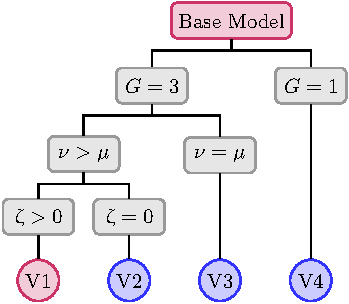
\includegraphics[width=0.8\linewidth]{variant-tree}
%  \caption{Summary of the Full model (F) and three model variants (V)
%    with respect to heterogeneity in risk, population growth (pop. growth), and turnover.
%    Relative population size of each risk group is the same in all variants.
%    $G$:~number of risk groups,
%    $\nu$:~rate of population entry,
%    $\mu$:~rate of population exit,
%    $\phi$:~rates of population turnover.}
%  \label{fig:variant-tree}
%\end{figure}
% \citep{Watts2010}: only model core group (FSW & Clients)
\color{black}